\cotefile{16}
\scanpage{53}

Supposons $k\geq0$, et le lemme prouvé pour $k'<k$. On sait déjà que les $p_i:H^*(X)\mathbin{-}H^i(X)$ sont $\in\operatorname{Alg}$ pour $i<k$, donc (transp.) pour $i>2n-k$. Soit
\[
T_k=\operatorname{id}-\sum_{i<k}p_i-\sum_{j>2n-k}p_j,
\]
donc $T_k\in A$, plus gén. $T_{k'}\in A$ si $k'\leq k$. Alors $\zeta^{n-k}T_k$ est nul sur $H^j$, $j\neq k$, et induit
\diagram{\begin{tikzcd}[ampersand replacement=\&]
H^k\arrow[r,"\zeta^{n-k}","\sim"']\&H^{2n-k}
\end{tikzcd}}
, donc $u_k\zeta^{n-k}T_k=p_k$.

D'autre part, si $i+2j=k$, \inserted{$j>0$,} la projection sur $\zeta^jP^i$ est aussi $\in A$, comme on voit \deleted{aussitôt} par récurrence ascendante sur $i$ (donc descendante sur $j$) ainsi : si $i<0$ rien à prouver. Si c'est fait pour les $i'<i$, on forme $\zeta^{n-k+j}T_k$, \deleted{$\unsure{\zeta}$} qui induit zéro sur $H^\alpha$ pour $\alpha\neq k$, et induit
\diagram{\begin{tikzcd}[ampersand replacement=\&]
H^k\arrow[r,"\zeta^{n-k-j}"]\&H^{2n-k+2j}
\end{tikzcd}}
, qui est nul \deleted{sur,} sur les facteurs $\zeta^{j'}P^{i'}$ pour $j'<j$, \inserted{de noyau $N$,} et sur les facteurs $\zeta^{j'}P^{i'}$ avec $j'\geq j$ (i.e. $i'\leq i$), \deleted{coïncide à $1$} dont la somme n'est autre que $\zeta^jH^{k-2j}$, son composé avec l'isom
\diagram{\begin{tikzcd}[ampersand replacement=\&]
H^{k-2j}\arrow[r,"\zeta^j","\sim"']\&\zeta^jH^{k-2j}
\end{tikzcd}}
est $\zeta^{n-(k-2j)}$. Donc l'hom $u_{k-2j}\zeta^{n-k+j}T_k$ \unsure{est}, nul sur $N$, et sur $\zeta^jH^{k-2j}$ l'inverse de
\diagram{\begin{tikzcd}[ampersand replacement=\&]
H^{k-2j}\arrow[r,"\sim"]\&\zeta^jH^{k-2j}
\end{tikzcd}}
. Donc

\mspage{52}

\cotefile{120}
\scanpage{2}
\margin{\unsure{1978|1778}}
\uline{\deleted{\unsure{Structure|Structures}}\inserted{Topologie} modérée}

(Autour de l'Eloge)
\mspage{1}

\scanpage{3}
\mspage{1}
\margin{\textcircled{I}\par\uline{Modèles \inserted{$R$-}modérés} \deleted{et espaces}\inserted{ens} \deleted{modérés}}
\[
\forall n\in\mathbb N^*,\qquad\mathcal M_n\subset\mathcal P(R^n)
\]
\textcircled{\scriptsize$M1$} $\forall u:[1,n]\longrightarrow[1,m]$, d'où $u^*:R^m\longrightarrow R^n$, on a
\[
u^*(\mathcal M_m)\subset\mathcal M_n\qquad\text{i.e.}\quad\forall A\in\mathcal M_m,\text{ on a }u^*(A)\in\mathcal M_n.
\]
\textcircled{\scriptsize$M2$} $\forall u:[1,n]\longrightarrow[1,m]$ \uline{surjectif}, d'où $u^*:R^m\hookrightarrow R^n$ injectif, on a
\[
u^{*-1}(\mathcal M_n)\subset\mathcal M_m\qquad\text{i.e.}\quad\forall \inserted{B}\in\mathcal M_n,\text{ on a }u^{*-1}(\deleted{A}\inserted{B})\in\mathcal M_m.
\]
\margin{donc si on a $M1$, on trouve\par $A\in\mathcal M_m\Longleftrightarrow u_*(A)\in\mathcal M_n$}
\textcircled{\scriptsize$M3$} $\forall u:[1,n]\longrightarrow[1,m]$ d'où $u^*:R^m\longrightarrow R^n$, et pour $A\in\mathcal M_m$, $B\in\mathcal M_n$, on a
\[
u^{*-1}(B)\cap A\in\mathcal M_m
\]
\textcircled{\scriptsize$M4$} $\forall A\in\mathcal M_m$, $B\in\mathcal M_n$, on a (modulo $R^m\times R^n\simeq R^{m+n}$)
\[
A\times B\in\mathcal M_{m+n}.
\]

\uline{Commentaires} \textcircled{1} $M1)$ permet de définir, pour \deleted{tout} $I$ ens fini non vide, $\mathcal M_I\in\mathcal P(R^I)$, et alors on a des propriétés $M'1$ à $M'4$ pour les $\mathcal M_I$ et les $u:I\mathbin{-}J$.

\textcircled{2} : Pour avoir $M1$, il suffit de le supposer pour les \deleted{trois} cas :

a) $m=n$, $u\in\mathfrak S_n$

b) $m=n+1$, $u$ injectif (``op. face''), donc $u^*$ surjectif

c) $n=m+1$, $u$ surjectif \deleted{\unsure{(``op. dégénérescence'')}} \inserted{(``op dégénérescence'')} donc $u^*$ injectif

\deleted{et $\overline{\mathrm m}$ seulement les \unsure{opérat\textsuperscript{s}|opérations} stand.}

\margin{ou $\overline{\mathrm m}$ seulement les op. standard\par
$R^n\mathbin{-}R^{n+1},\ (x_1,\ldots,x_n)\longmapsto(x_1,\ldots,x_n,x_n)$\par
et\par
$R^{n+1}\mathbin{-}R^n,\ (x_1,\ldots,x_{n+1})\longmapsto(x_1,\ldots,x_n)$}

Pour avoir $M2$, il suffit de le supposer pour les op${}^{\mathrm{o}}$ de dégénérescences, \inserted{et $\overline{\mathrm m}$ seulement pour l'application \deleted{$\unsure{R^n\hookrightarrow R^{n+1}}$} \figure{
\begin{tikzpicture}[x=.12cm,y=.12cm,baseline=-.5ex]\draw[line width=1.2pt] (0,0)--(.7,3) (.45,1.1)--(1.6,.2)--(.3,.6)--(1.1,1.6);\end{tikzpicture}}}
\margin{\figure{
\begin{tikzpicture}[x=.12cm,y=.12cm]\draw[line width=1.2pt] (0,0)--(.7,3) (.45,1.1)--(1.6,.2)--(.3,.6)--(1.1,1.6);\end{tikzpicture}}\par
\figure{\begin{tikzpicture}[x=1cm,y=1cm]
\draw (-2.05,.95) .. controls (-.5,.92) and (2.1,1) .. (2.15,.25)
 .. controls (2.45,-.8) and (1.95,-1.05) .. (.1,-1.05)
 .. controls (-2.15,-1.02) and (-2.25,-.6) .. (-2.05,.95);
\node at (0,0) {$\begin{gathered}R^n\hookrightarrow R^{n+1}\\(x_1,\ldots,x_n)\deleted{\unsure{\longmapsto|x_n}}\\\longmapsto(x_1,\ldots,x_n,x_n)\end{gathered}$};
\end{tikzpicture}}}
Notons que $M1$, $M2$, $M4$ impliquent que les $\mathfrak S_n$ sont stables par intersection de deux
\[
A,B\in\mathfrak S_n\Longrightarrow A\cap B\in\mathfrak S_n
\]
\inserted{(moyennant $M1$, $M2$, $M4$)}
d'où résulte que pour avoir $M3$, il suffit de le prouver pour $u$ injectif, et $\overline{\mathrm m}$ seulement pour $u^*$ l'op. standard
\[
R^{n+1}\mathbin{-}R^n,\quad(x_1,\ldots,x_{n+1})\longmapsto(x_1,\ldots,x_n).
\]
\mspage{2}

\scanpage{4}
En résumé on voit que $M1$, $M2$, $M3$ peuvent être remplacés par

a) \deleted{$\forall n\ \forall\sigma\in\mathfrak S_n$} $\forall n\in\mathbb N^{*}$, $\sigma\in\mathfrak S_n$, $A\in\mathcal M_n$, on a $\sigma^*(A)\in\mathcal M_n$

b) $\forall n\in\mathbb N^*$, d'où
\[
\alpha_n:[1,\ldots n+1]\longrightarrow[1,n]\qquad
\left\{\begin{gathered}\text{identité sur }[1,n]\\ n+1\mathrel{\mapstochar\relbar}n\end{gathered}\right.
\]
d'où \deleted{$R$}
\[
\alpha_n^*:R^n\hookrightarrow R^{n+1}\qquad(x_1,\ldots,x_n)\longmapsto(x_1,\ldots,x_n,x_n),
\]
on a
\[
\begin{aligned}
b_1)\quad&\forall A\in\mathcal M_n,\quad\alpha_n^*(A)\in\mathcal M_{n+1},\\
b_2)\quad&\forall B\in\mathcal M_{n+1},\quad\alpha_n^{*-1}(B)\in\mathcal M_n
\end{aligned}
\]
c) $\forall n\in\mathbb N^*$, d'où $\beta_n:[1,n]\hookrightarrow[1,n+1]$ inclusion can., d'où
\[
\beta_n^*:R^{n+1}\longrightarrow R^n,\quad(x_1,\ldots,x_{n+1})\mathrel{\mapstochar\relbar}(x_1,\ldots,x_n),
\]
on a
\[
\begin{aligned}
c_1)\quad&\forall A\in\mathcal M_{n+1},\ B\in\mathcal M_n,\text{ on a }A\cap\beta_n^{*-1}(B)\in\mathcal M_{n+1}\\
c_2)\quad&\forall A\in\mathcal M_{n+1},\quad\beta_n^*(A)\in\mathcal M_n
\end{aligned}
\]

\textcircled{3} $M1$ implique que si un des $\mathcal M_n$ est vide, tous le sont -- et alors les axiomes $M1$ à $M4$ sont satisfaits trivialement. On va exclure ce cas \inserted{trivial}, i.e. supposer
\[
(*)\qquad\mathcal M_1\ne\varnothing.
\]
$M1$ implique que si un des $\mathcal M_n$ contient $\varnothing$, tous le contiennent. Si ce n'est pas le cas, alors chaque $\mathcal M_n$ (étant stable par intersection de deux ens) est une base de filtre sur $R^n$.

On exclut ce cas, i.e. on suppose la relation suivante, plus forte que $(*)$
\[
(**)\qquad\varnothing\in\mathcal M_1\qquad(\text{d'où }\varnothing\in\mathcal M_n\quad\forall n\in\mathbb N)
\]
\uline{NB} Si cette propriété n'étant vérifiée, alors posant
\mspage{3}

\scanpage{5}
\mspage{2}
\[
\mathcal M'_n=\mathcal M_n\cup\{\varnothing\}
\]
les $\mathcal M'_n$ satisfont encore les axiomes \ldots

\deleted{\textcircled{4} On a NB Si on pose}

De $\overline{\mathrm m}$, \deleted{$M$} $M1$ implique que si on a, pour \uline{un} $n$, \deleted{$M$} $\mathcal M_n=\{\varnothing\}$, alors c'est vrai aussi pour $\forall n$ -- cas trivial \inserted{(qui satisfait aux axiomes)} que je vais exclure. Donc je suppose aussi
\[
(***)\quad\deleted{\exists}\ \mathcal M_1\ne\{\varnothing\}\quad\text{i.e.}\quad\exists A\in\mathcal M_1,\quad A\ne\varnothing.
\]
Ceci étant, si on pose pour \inserted{$I\ne\varnothing$}
\[
\mathcal M_\varnothing=\mathcal P(\underbrace{R^\varnothing}_{\text{espace ponctuel }\{e\}})=\{\varnothing,\{e\}\}
\]
\margin{les propriétés $M'1$ à $M'4$ (cf \textcircled{1}) restent satisfaites sans se borner à \deleted{$I,J\unsure{\ne\varnothing}$} $I,J\ne\varnothing$ \ldots}

\textcircled{4} Soit \deleted{$x\in R^n$}
\[
x=(x_1,\ldots,x_n)\in R^n
\]
alors il résulte de $M1$ et $M4$ que
\[
\{x\}\in R^n\Longleftrightarrow\forall i\in[1,n],\text{ on a }\{x_i\}\in\mathcal M_1.
\]
Soit
\[
R_0=\{x\in R\mid\{x\}\in\mathcal M_1\}\qquad\text{donc }R_0\subset R,
\]
alors pour tt ens fini $I$, on a
\[
\begin{array}{l}
R_0^I=\{a\in R^I\mid\{x\}\in\mathcal M_I\}\\
\cap\\
R^I
\end{array}
\]
Notons que si \deleted{$R_0\ne\varnothing$} \inserted{$\mathrm{Card}\ R_0\ge2$}, alors on conclut de la stabilité \inserted{de $\mathcal M_1$} par intersection que $\varnothing\in\mathcal M_1$, donc on satisfait à \textcircled{3}.

\textcircled{5} Exemples (à part $\mathcal M_n=\varnothing\quad\forall n$, et $\mathcal M_n=\{\varnothing\}\quad\forall n$)
\mspage{4}

\scanpage{6}
a) $\mathcal M_n=$ parties de cardinal $\le1$ de $R^n$

b) $\mathcal M_n=$ parties finies de $R^n$

c) $\mathcal M_n=$ toutes les parties de $R^n$

Aucun de ces exemples \unsure{n'est} \unsure{intéressant} pour nous!

\margin{\textcircled{II} \uline{espaces modérés}\par
Dans ce qui suit au lieu de $(M1)$ il suffit l'axiome concernant \deleted{\unsure{les injections}} \inserted{les surjections} \unsure{particulières} \uline{pour les seuls} $[1,n]$ -- c.-à-d. les \unsure{axiomes de stabilité} \illegible{2} applications diagonales, et \unsure{pas les} \uuline{images} directes.}
\margin{ici les axiomes a), b), c) du NB \textcircled{2}, \uline{à l'exclusion} de $c_2)$}
\margin{on n'exclut pas $I$ vide}

Terminologie : partie modérée de $R^I$, points modérés de $R$, de $R^I$.

\uline{déf} Soit $A\in\mathcal M_I$, $B\in\mathcal M_J$, $f:A\mathbin{-}B$, d'où
\[
\Gamma_f\subset A\times B\subset R^I\times R^J\simeq R^{I\cup J}.
\]
On dit que $f$ est \uline{modérée} si
\[
\Gamma_f\in\mathcal M_{I\cup J}.
\]

\margin{via $M2$}
\uline{Proposition} a) $\mathrm{id}_A$ (si $A\in\mathcal M_I$) est modérée

b) \diagram{\begin{tikzcd}[row sep=tiny,column sep=large]
f:A\arrow[r,no head]&B&\text{et}&g:B\arrow[r,no head]&C\\
\mathcal M_I\arrow[u,phantom,"\rotatebox{90}{\(\in\)}" description]&\mathcal M_J\arrow[u,phantom,"\rotatebox{90}{\(\in\)}" description]&&&\mathcal M_{K}\arrow[u,phantom,"\rotatebox{90}{\(\in\)}" description]
\end{tikzcd}} modérés $\Longrightarrow gf$ modéré

c) \diagram{\begin{tikzcd}[row sep=tiny]
f:A\arrow[r]&B\\
\mathcal M_I\arrow[u,phantom,"\rotatebox{90}{\(\in\)}" description]&\mathcal M_J\arrow[u,phantom,"\rotatebox{90}{\(\in\)}" description]
\end{tikzcd}} modéré et bijectif $\Longrightarrow f^{-1}$ modéré

D'où catégorie des \uline{modèles modérés} $\mathrm{Mod}_{\mathcal M_*}$, \inserted{(on prend $(I,A\in\mathcal M_I)$)} et un foncteur \uline{conservatif} \uline{fidèle}
\diagram{\begin{tikzcd}
\mathrm{Mod}_{\mathcal M_*}\arrow[r]&(\mathrm{Ens})
\end{tikzcd}}\qquad$(I,A)\longmapsto A$.
\margin{on n'exclut pas les modèles $\subset R^0=\{e\}$, \inserted{modèle} \deleted{espace} réduit à un point \ldots}

On en déduit\deleted{\unsure{on}} la catégorie des ensembles \inserted{(ou ``espaces'')} $(\mathcal M_*-)$ modérés, équivalente : $\mathrm{Mod}_{\mathcal M_*}$, mais avec un foncteur
\diagram{\begin{tikzcd}
\deleted{\unsure{\mathrm{Mod}}}\ \mathrm{Esp}_{\mathcal M_*}\arrow[r]&(\mathrm{Ens})
\end{tikzcd}}\qquad$X\mathrel{\mapstochar\relbar}|X|$
qui est fidèle, conservatif et de plus ``transportable'', i.e.
\mspage{5}

\scanpage{7}
\mspage{6}\hfill\mspage{3}
pour tout diagramme
\diagram{\[
\left\{\begin{gathered}\begin{tikzcd}[row sep=large]
\deleted{A}\inserted{X}&\\
{|X|}\arrow[r,"{\substack{\alpha\\\sim}}"]&E
\end{tikzcd}\end{gathered}\right.
\]}
avec $X\in\mathrm{Ob}\,\mathrm{Esp}_{\mathcal M_*}$, $\exists$ une unique \deleted{$Y$ et} flèche $f:X\mathbin{-}Y$ de $\mathrm{Esp}_{\mathcal M_*}$, qui relève $\alpha$ (``Transport de structure'').

\uline{Proposition} Dans la catégorie $\mathrm{Esp}_{\mathcal M_*}$ des espaces $\mathcal M_*$-modérés, il y a des
\deleted{produits fibrés \inserted{\deleted{(de deux objets} sur un troisième)}, et des produits (de deux objets), et le foncteur $X\mathrel{\mapstochar\relbar}|X|$ y commute. Si on suppose
\[
(M5)\qquad R_0\ne\varnothing
\]
alors il \deleted{foncteur} y a aussi un objet final (qui est uniponctuel) et le foncteur}
\inserted{des limites finies}
et le foncteur $X\mathrel{\mapstochar\relbar}|X|$ y commute.
\margin{\unsure{trivialité de} \unsure{suivi} d'un \illegible{1} \unsure{et des} \illegible{2} des \unsure{foncteurs}}

\uline{Proposition} Si pour \uline{un} $n\in\mathbb N^*$ on a \deleted{$\unsure{R}$} $R^n\in\mathcal M_n$, alors c'est vrai pour $\forall n$, et même pour $\forall I$ fini \inserted{dans}
\[
R^I\in\mathcal M_I.
\]
Considérons l'axiome (\uline{facultatif})
\[
\deleted{\unsure{M5}}(M0)\qquad R\in\mathcal M_1\qquad(\Longrightarrow\forall I\in(\mathrm{Ens\ fini}),\ R^I\in\mathcal M_I)
\]
\margin{Quand on n'a pas $(M0)$, mais que l'on suppose $(M5)$, alors la réunion des $A\in\mathcal M_1$, fait que $\unsure{R'}$ est \unsure{obtenu} \unsure{comme} \illegible{2} \unsure{de} $\unsure{R}$ \unsure{réunion} \unsure{filtrante} \illegible{2} $\unsure{\mathcal E|\Sigma}$.\par
\unsure{On dispose} de \unsure{ces} \unsure{ens.} \unsure{stables} \illegible{2} l'axiome $(M1)$ \unsure{s'exprime} \illegible{1} \unsure{l'influence} \unsure{de} \unsure{foncteurs} \illegible{2}.\par
\unsure{comme} $(M5)$ l'expression \unsure{espace} \unsure{muni de} \unsure{l'} $\unsure{R}$ \unsure{aussi} \unsure{vide} \unsure{annulé}.}
\margin{\unsure{objet} \unsure{abs.} \unsure{Cat}\uline{\unsure{f}}}

\scanpage{8}
Alors $R$ est muni d'une structure modérée canonique (en tant que modèle $\subset R^1=R$), i.e.
\[
 R\in\operatorname{Ob}\mathcal E\qquad(\mathcal E=\operatorname{Esp}_{\mathcal M_*})
\]
et $\forall$ objet de $\mathcal E$ est isomorphe à un sous-objet d'un $R^n$ \inserted{(produit dans $\mathcal E$)}. On récupère $\mathcal M_n$ comme l'ens des \inserted{sous-ens. de $R^n$ \unsure{correspondants dans Ens}} sous-objets (dans $\mathcal E$) de l'objet $R^n$. On trouve que la donnée d'un $\mathcal M_*$ est équivalente à la donnée d'un système (à isom. près)
\[
 (\mathcal E,R,X\mathrel{\mapstochar\relbar}|X|)
\]
de a) la catégorie $\mathcal E$ avec $\varprojlim$ finies

b) le foncteur $X\mathrel{\mapstochar\relbar}|X|$ $\mathcal E\mathbin{-}(\mathrm{Ens})$ exact à gauche

c) l'objet $R\in\operatorname{Ob}\mathcal E$ tel que tt objet de $R$ se plonge dans un $R^n$.

\margin{Parler aussi des applications modérées d'ens. modérés \uline{dans des $R^I$}.}

\margin{Introduire les parties modérées d'un espace modéré correspondant aux sous-objets dans $\operatorname{Esp}_{\mathcal M_*}$, les propriétés de stabilité $f(A)$, $f^{-1}(B)$, produits cartésiens.}

\figure{\begin{tikzpicture}\node[draw,ellipse] {III};\end{tikzpicture}}
\uline{Limites inductives finies d'espaces modérés}

S'intéresser à la question des réunions finies des parties modérées, et des $\varinjlim$ finies dans $(\operatorname{Esp}_{\mathcal M_*})$.

\margin{A partir d'ici, on suppose que $\unsure{M4|M5}$ de réunion seulement \unsure{possible}. Je verrai \uline{bien} $(M1)_0$ pour la suite par un axiome.}
\mspage{7}

\scanpage{9}
\mspage{4}
\margin{le donner \uline{après} la proposition qui suit, ou postuler\ldots}
\uline{Proposition} Si \deleted{$R_0\ne\varnothing$}, \inserted{$\operatorname{Card}R_0\geq2$}, \deleted{alors \unsure{(si} \inserted{$(\unsure{\Leftrightarrow}R\in\mathcal M_1)$}, $\mathcal E$ dans} $\mathcal E$
\deleted{existe un \illegible{1}\inserted{$(\operatorname{Hom}_{\mathcal E}(\unsure{e''|e},R))$} de l'objet \unsure{$R_0$}}
\deleted{$\operatorname{Hom}_{\mathcal E}(\underset{\inserted{\substack{\shortparallel\\\{e\}}}}{R^0},R)\ne\varnothing$)} dans des
\deleted{$\mathcal E$ il y a des sommes finies} (moyennant \figure{\begin{tikzpicture}[baseline=(m.base)]\node[draw,ellipse,inner sep=1pt] (m) {$M5$};\end{tikzpicture}} et $X\mathrel{\mapstochar\relbar}|X|$ y commute.

\uline{Corollaire} Sur $\forall$ ens fini il $\exists$ une structure modérée et une seule, pour laquelle les parties uniponctuelles soient modérées (str. mod. discrète).

\unsure{On se propose} le cas où on veut construire $X_1\amalg_Z X_2$, sans supposer $Z$ vide. Notons d'abord ceci :

\uline{Proposition} Soit $I$ un \deleted{type de} \inserted{type de} diagrammes fini, et $(X_i)_{i\in I}$ un diagramme de type $I$ dans $\mathcal E=\operatorname{Esp}_{\mathcal M_*}$, i.e. d'espaces modérés. Soit $X$ la limite inductive \uline{dans} $(\mathrm{Ens})$, qui est donc un \inserted{certain} quotient de $\coprod X_i$ (comme toujours). Supposons qu'il existe sur $X$ une structure modérée, telle que les appl. can. $g_i:X_i\longrightarrow X$ soient modérées. Alors $X$, muni de cette structure, est \inserted{une} $\varinjlim_I$ des $X_i$.
\mspage{8}

\scanpage{10}
Axiome supplémentaire
\[
 (M5)\quad \forall n,\quad \mathcal M_n\text{ stable par réunions finies}
\]
\[
 (\Longleftrightarrow\ \varnothing\in\mathcal M_n,\ \deleted{\unsure{\delta}}\text{ et }A,B\in\mathcal M_n\Longrightarrow A\cup B\in\mathcal M_n)
\]
\uline{Proposition} Parties modérées d'un esp. mod. stable par réunions finies.

\uline{Proposition} Sur $\varnothing$ il y a une structure modérée unique, qui en fait objet initial de $\operatorname{Esp}_{\mathcal M_*}$.

\uline{Proposition} Soient $X$ un espace modéré, $(X_i)_{i\in I}$ une famille finie de parties modérées de $X$. Alors $\bigcup X_i$ est une partie modérée de $X$. Si $X=\bigcup_iX_i$, alors $X$ est somme amalgamée des $X_i$ suivant les $X_i\cap X_j$ --- une application $f:X\longrightarrow Y$ \inserted{entre espaces modérés} est modérée ssi ses restrictions aux $X_i$ le sont.

\uline{Question} Donnons-nous
\diagram{\begin{tikzcd}[column sep=small]
&\deleted{Y}\inserted{Z}\arrow[dl,hook']\arrow[dr,hook]&\\
X_1&&X_2
\end{tikzcd}}
dans $\operatorname{Esp}_{\mathcal M_*}$, existe-t-il une somme amalgamée ? Si $Y=\varnothing$, c'est la question de l'existence des sommes finies dans $(\operatorname{Esp}_{\mathcal M_*})$.
\mspage{9}

\scanpage{11}
\mspage{5}
Pour que la somme amalgamée existe dans \deleted{$\operatorname{Esp}$} $\mathcal E$ et que $X\mathrel{\mapstochar\relbar}|X|$ y commute, il f. et s. qu'il existe une famille finie de \inserted{paires de} fonctions
\[
\begin{array}{l}
f_\alpha:\deleted{g}\ X_1\mathbin{-}R\\
g_\alpha:X_2\mathbin{-}R
\end{array}
\]
telles que l'on ait
\[
\text{a)}\quad f_\alpha(i_1(z))=g_\alpha(i_2(z))\qquad\forall\alpha\in A,\ z\in Z
\]
b) \deleted{Si $x,y$ les $f_\alpha$ \unsure{x} $(f_\alpha):$} les $f_\alpha$ ($g_\alpha$) séparent les pts de $X_1$ ($X_2$) i.e.
\[
 X_1\mathbin{-}R^I\qquad(X_2\mathbin{-}R^A)
\]
sont injectifs
\[
\begin{array}{ll}
\text{c)}&\text{Si }x_1\deleted{\unsure{\alpha}}\in X_1\smallsetminus i_1(Z)\\
&x_2\in X_2\smallsetminus i_2(Z)\\
&\exists\alpha\text{ avec }f_\alpha(x_1)\ne g_\alpha(x_2)
\end{array}
\]

\uline{NB} On peut généraliser, sous les conditions de la proposition, il existe la structure modérée qu'on veut sur $X$, ssi $\exists$ une famille finie $(F_\alpha)$ \deleted{de} de systèmes inductifs
\[
 (f_{\alpha i})_{i\in I}\qquad f_{\alpha i}:X_i\underset{\text{modérée}}{\longrightarrow}R),
\]
obtenant des
\[
 f_\alpha:X\longrightarrow R
\]
telles que les $f_\alpha$ séparent les pts de $X$, i.e.
\[
 f=(f_\alpha):X\hookrightarrow R^A
\]
\mspage{10}

\scanpage{12}
En effet, si $Y$ est un espace modéré, une \deleted{biject.} \unsure{flèche} du syst. inductif $(X_i)$ (dans $\mathcal E$) dans $Y$, \inserted{$(f_i:X_i\mathbin{-}Y)_{i\in I}$}, équivaut à la donnée d'une application $f:X\mathbin{-}Y$, telle que les $f\circ g_i$ soient modérées. Il est \unsure{évident} : prouvons que cela implique que $f$ est modérée, i.e. que son graphe $\Gamma_f\subset X\times Y$ est une partie modérée. Or $X$ étant la réunion des images des $X_i$, il en est que $\Gamma_f$ est la réunion des images des $\Gamma_{f_i}\subset X_i\times Y$ par
\[
 X_i\unsure{\deleted{\times Y}|\times Y}\xrightarrow{g_i\times\operatorname{id}_Y}X\times Y.
\]
Mais ces images sont modérées, et donc leur réunion aussi.

\uline{Cor} Soit $f:X\longrightarrow Y$ application modérée, $\mathcal R_f$ la relation d'équivalence définie par $f$ (qui est donc une partie modérée de $X\times X$, et est une $\mathcal E$-relation d'équivalence). Alors $X/\mathcal R_f$ existe dans $\mathcal E=\operatorname{Esp}_{(\mathcal M_*)}$, et est \inserted{can} isomorphe à $f(X)$ (avec structure induite)

\deleted{\uline{Cor. 2} Considérons}
\deleted{\diagram{\begin{tikzcd}[column sep=small]
&\deleted{Z}\arrow[dl,hook',"\deleted{i_1}"']\arrow[dr,hook,"\deleted{i_2}"]&\\
\deleted{X_1}&&\deleted{X_2}
\end{tikzcd}}}
\deleted{dans $\mathcal E$.}
\mspage{11}

\scanpage{13}
\mspage{6}
On va introduire
\[
(M6)\quad\deleted{\unsure{\exists f_\alpha}}\quad
\left\{\begin{aligned}
&\forall \deleted{\unsure{X}}\inserted{Z},X\in\mathcal M_n,\quad Z\subset X,\quad\exists(f_\alpha)_{\alpha\in A}\ \text{famille}\\
&\text{finie de fonctions modérées }X\longrightarrow R\\
&\text{et des }(e_\alpha)_{\alpha\in A},\quad e_\alpha\in R_0,\quad\text{telle que}\\
&Z=\bigcap f_\alpha^{-1}(e_\alpha).\quad\text{De plus, OPS que les}\\
&f_\alpha\text{ séparent les points de }X\smallsetminus Z.
\end{aligned}\right.
\]

\margin{\uline{Prop} $(M6)$, $(M7)$ impliquent l'existence de la somme amalg. avec une flèche libre.}
\margin{\diagram{\begin{tikzcd}[column sep=small]
X_1&Z\arrow[l,hook']\arrow[r]&X_2
\end{tikzcd}}}

\deleted{Cela implique que l'on peut faire un diagramme \inserted{cart}}
\deleted{\diagram{\begin{tikzcd}
\deleted{X}\arrow[r,hook]&\deleted{R^n\times R^A}\\
\deleted{Z}\arrow[u,hook]\arrow[r,hook,no head]&\deleted{R^n\times\{e\}}\arrow[u,hook]
\end{tikzcd}}}
\deleted{$e=(e_\alpha)_{\alpha\in A}$}

\deleted{Appliquons ceci : $Z_1\hookrightarrow X_1$ et $Z_2\mathrel{\lhook\joinrel\relbar}X_2$}

ce qui \uline{équivaut} au fait que le quotient $X/Z$ (contraction de $Z$ en un point) existe dans $\mathcal E$ au sens strict (i.e. $X\mathrel{\mapstochar\relbar}|X|$ y commute). De plus, on suppose
\margin{\unsure{supplém.} important)}
\[
(M7)\quad\forall Z,X\in\mathcal M_n,\quad Z\subset X,\quad\text{et tte}
\]
\[
f:Z\longrightarrow R\text{ modérée},\qquad\exists g:X\longrightarrow R\text{ modérée}
\]
qui prolonge \unsure{$f$}

\uline{Proposition} Moyennant $M5,M6,M7$, les sommes amalgamées $X_1\amalg_Z X_2$ ($Z\hookrightarrow X_1$, $Z\hookrightarrow X_2$) existent dans $\operatorname{Esp}_{\mathcal M_*}$, et commutent au foncteur oubli\ldots
\margin{cf généralisation qui vient ci-dessous.}
\mspage{12}

\scanpage{14}
Soit $Z\mathrel{\lhook\joinrel\relbar}R^{\deleted{\unsure{n}}\inserted{I}}$ un plongement modéré. On peut (par $M7$) le prolonger en
\[
 X_i\longrightarrow R^I\qquad(i\in\{1,2\})
\]
Soit \unsure{(}
\[
 X_i\mathbin{-}R^{A_i}\qquad i\in\{1,2\}
\]
comme dans $M6$ (d'où un \deleted{\unsure{appl.}} plongement modéré $X_i/\underset{\inserted{=u_i(Z)}}{Z_i}\mathrel{\lhook\joinrel\relbar}R^{A_i}$), \deleted{\unsure{on}}\inserted{on} a donc un : $X_1\longrightarrow R^{I\amalg A_1}$ qui est un plongement et s'insère dans un diagramme cartésien
\par\noindent\diagram{\begin{tikzcd}
X_1\arrow[r,hook,no head]&R^{I\amalg A_1}=R^I\times R^{A_1}\\
Z\arrow[u,hook,no head]\arrow[r,hook,no head]&R^I\times\{e_1\}\arrow[u,hook]&e_1\in R_0^{A_1}
\end{tikzcd}}\par
et de $=$ pour $X_2$, \deleted{on le} qu'on peut considérer comme \deleted{\unsure{des|dans}} s'insérant dans
\deleted{\par\noindent\diagram{\begin{tikzcd}[column sep=small]
\deleted{X_1}\arrow[r,hook,no head]\arrow[d,no head]&\deleted{R^I\times R^{A_1}\times\{e_2\}}\arrow[r]\arrow[d]&\deleted{R^I\times R^{A_1}\times R^{A_2}}\\
\deleted{Z}\arrow[r]&\deleted{R^I\times\{e_1\}\times\{e_2\}}&\deleted{R^I\times R^{A_2}\times R^{A_2}}\arrow[u]
\end{tikzcd}}\par}
\par\noindent(*)\quad\diagram{\begin{tikzcd}[column sep=small,row sep=small]
X_1\arrow[r,hook]&R^I\times R^{A_1}\times\{e_2\}\arrow[r,hook,no head]&R^I\times R^{A_1}\times R^{A_2}\\
& R^I\times\{e_1\}\times\{e_2\}\arrow[u,hook]\arrow[r,hook]&R^I\times\{e_1\}\times R^{A_2}\arrow[u,hook,no head]\\
\deleted{R}\inserted{Z}\arrow[uu,hook]\arrow[rr,hook]&&X_2\arrow[u,hook,no head]
\end{tikzcd}}\par
\mspage{13}

\scanpage{15}
\mspage{14}\mspage{7}
\margin{on suppose $M5$ mais pas $M6$ ni $M7$\ldots}
\figure{\begin{tikzpicture}\node[draw,ellipse] {$\overline{\underline{\mathrm{IV}}}$};\end{tikzpicture}}
Ind-structures modérées strictes \inserted{\uline{indespaces $\overset{\overline{\longrightarrow}}{\text{modérés}}$}} \inserted{(ou ind-espaces modérés)} : \unsure{consiste} : la donnée d'un ens. $E$, et un ens de parties $\mathcal M_E$ sur $E$ (les parties modérées), stable par réunions finies, \inserted{de réunion $E$}, avec une structure modérée sur chacun, ces structures s'induisant mutuellement, et
\[
 A\in\mathcal M,\quad B\in\mathcal M_A\Longrightarrow B\in\mathcal M.
\]
Il revient au $=$ de se donner la notion d'application modérée d'un $X$ modéré dans $E$, avec \deleted{une identité} quelques conditions supplém.. Si on suppose
\[
 (M8)\quad R\text{ est réunion \inserted{(filtrante par $M5$)} de ses parties modérées},
\]
on trouve une structure ind-modérée canonique sur $R$, et de $=$ sur les $R^I$.

\uline{Proposition} La catégorie des \inserted{$\overset{\leftrightarrow}{\underrightarrow{\operatorname{Esp}}}_{\mathcal M_*}$} \deleted{Ind} Ind-espaces modérés stricts admet des $\varprojlim$ finies, le foncteur oubli y commute.
\margin{\unsure{des ensembles modérés|des ind-modérés}}
\margin{$M1:M5$}
\margin{$\underrightarrow{\operatorname{Esp}}_{\mathcal M_*}$ est obtenue par $\uline{\varinjlim}$ filtrantes \unsure{des injections} \deleted{strictes} \unsure{dans les ensembles} \unsure{modérés} \unsure{quelconques}.}

Si $R_0\ne\varnothing$ (idem dans $\underrightarrow{\operatorname{Esp}}_{\mathcal M_*}$ il y a sommes disjointes finies) il y a des sommes disjointes \deleted{finies} \inserted{(en principe !)} dans $\overset{\leftrightarrow}{\underrightarrow{\operatorname{Esp}}}_{\mathcal M_*}$, et $X\longrightarrow |X|$ y commute.

\scanpage{16}
Soit $\deleted{\unsure{E}}\inserted{\mathcal X}$ un espace ind-modéré. Une partie \deleted{$\mathcal Y$} de $\mathcal X$ est dite loc. modérée si $\forall A\in\mathcal M_{\mathcal X}$, on a $A\cap\mathcal Y\in\mathcal M_{\mathcal X}$. C'est stable par intersections finies (y compris pour famille vide, i.e. $\mathcal X\in\unsure{\underrightarrow{\overrightarrow{\mathcal M}}|\underrightarrow{\widetilde{\mathcal M}}}_{\mathcal X}$), par image inverse par morphismes \deleted{loc.} d'espaces ind-modérés.

La notion d'application modérée d'un espace modéré $X$ dans un $R^I$, est un cas particulier de la précédente, quand $M8$ est satisfait donc $X$ et $R^I$ sont tous deux des espaces ind-modérés.

Moyennant $M6,M7$, il existe \deleted{pour} dans $\underrightarrow{\operatorname{Esp}}_{\mathcal M_*}$ le quotient $\mathcal X/\mathcal Y$ au sens (et commute : $X\mapsto|X|$), si $\mathcal Y$ est partie $\mathrm{loc}^{\mathrm t}$ modérée, et de $=$
\[
 \mathcal X_1\amalg_{\mathcal Z}\mathcal X_2
\]
pour $\mathcal Z\lhook\joinrel\relbar\mathcal X_1$ et $\mathcal Z\lhook\joinrel\relbar\mathcal X_2$ des ``immersions modérées'' i.e. correspondant à des parties \inserted{loc} modérées.
\mspage{15}

\scanpage{17}
\mspage{8}
$\mathcal Z_i\subset\mathcal X_i$ et $Z\simeq\mathcal Z_1$, $Z\simeq\mathcal Z_2$).

\uline{NB} On fera attention que contrairement à ce qui se passe dans $\deleted{\unsure{\operatorname{Cat}}}\inserted{\operatorname{Esp}}_{\mathcal M_*}$) un sous-objet d'un objet $\mathcal X$ de $\underrightarrow{\operatorname{Esp}}_{\mathcal M_*}$ i.e. d'un esp. ind-modéré, ne correspond pas néc. à une partie $\mathrm{loc}^{\mathrm t}$ modérée\ldots

\figure{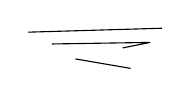
\begin{tikzpicture}\draw (0,0)--(1.7,.05);\draw (.3,-.15)--(1.55,-.13)--(1.2,-.2);\draw (.6,-.34)--(1.3,-.46);\end{tikzpicture}}
\figure{\begin{tikzpicture}\node[draw,ellipse] {$\overline{\underline{\mathrm V}}$};\end{tikzpicture}}
\uline{\unsure{Relations|Relation} aux topologies} Supposons $R$ muni d'une topologie, donc les $R^I$ et les ``modèles'' modérés aussi. On voudrait que les applications modérées soient continues --- c'est OK si les parties modérées sont compactes (donc fermées, si $R$ séparé), c'est le cas. \deleted{Si le foncteur $X\mathrel{\mapstochar\relbar}$} \inserted{Supposons donc}
\figure{\begin{tikzpicture}\node[draw,ellipse] {$M9$};\end{tikzpicture}}
\[
 \left\{\begin{array}{l}R\text{ séparé}\\
 \text{les parties modérées de }R^n\text{ sont compactes}
 \end{array}\right.
\]
Alors le foncteur $X\mathbin{-}|X|$ se factorise par la cat. des espaces topologiques
\[
 \operatorname{Esp}_{\mathcal M_*}\longrightarrow(\deleted{\unsure{R|E}}\inserted{\mathrm E}\mathrm{sp.\ top.\ cpts})
\]
\mspage{16}

\scanpage{19}
\mspage{9}
On voit \inserted{alors} que l'on a la notion d'application $X\longrightarrow Y$ entre espaces modérés, qui est \uline{modérée au voisinage d'un pt}, et on trouve

\uline{Prop} Pour qu'une application d'un espace modéré $X$ dans un espace ind-modéré soit modérée, il faut s. qu'elle le soit au voisinage de chaque pt.

Donc les applications modérées de $X$ dans $Y$ forment les sections d'un faisceau --- le faisceau des applications modérées de $X$ dans $Y$. La structure \inserted{modérée} de $X$ est connue quand on connaît l'ens des applications modérées de $X$ dans $R$ (cela \unsure{vaut|faut} dans le contexte purement ensembliste, avec $(M1)_0$\unsure{;|?} $(M2)$ $(M3)$ $(M4)$ seulement), donc aussi quand on connaît le faisceau des germes de fonctions modérées.
\mspage{18}

\scanpage{20}
\uline{Espace loc. modéré} Esp. \deleted{loc. cpct} \inserted{ind-modérés} dont la top. est \deleted{loc. cpcte} séparée, et tt point admet un \uline{voisinage} qui est \deleted{\unsure{esp.|cpt}} modéré (donc l'espace est loc. cpct), et tt pt admet un syst. fond. de voisinages modérés, et les parties compactes sont les parties contenues dans une partie modérée --- qui forment donc un antifiltre cofinal : celui des parties compactes.

Par exemple, par $(M10)$ $R$ est un espace $\mathrm{loc}^{\mathrm t}$ modéré, donc les $R^I$ aussi.

Les espaces loc. modérés \deleted{$\unsure{f}\ \operatorname{Esploc}_{\mathcal M_*}$} forment une sous-catégorie pleine $\operatorname{Esploc}_{\mathcal M_*}$ de $\underrightarrow{\operatorname{Esp}}_{\mathcal M_*}$, stable par $\varprojlim$ finies.

\margin{Dire qu'une partie compacte et \deleted{fermée} d'un espace modéré est modérée.}
\margin{\deleted{\unsure{loc.}}}
\figure{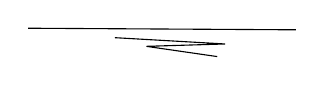
\begin{tikzpicture}\draw (0,0)--(3.4,-.02);\draw (1.1,-.12)--(2.5,-.2)--(1.5,-.23)--(2.4,-.36);\end{tikzpicture}}
\mspage{19}

\scanpage{21}
\mspage{20}\mspage{10}
\figure{\begin{tikzpicture}\node[draw,ellipse] {$\overline{\underline{\mathrm{VI}}}$};\end{tikzpicture}}
\margin{\uline{Relation avec structure de corps}}
Oublions les structures topologiques, supposons par contre que $R$ ait une \uline{structure de corps}. On supposera alors, \deleted{\unsure{Alrt}} en plus de $(M1)_{\unsure{0}}$ et $(M4)$ (minimum pour construire $\operatorname{Esp}_{\mathcal M_*}$ avec ses $\varprojlim$ finies) l'axiome

\deleted{$(M11)$ \deleted{a) Pour tt} partie modérée $A$ de $R$, l'application $a\mapsto-a$ de $A$ dans $R$ est modérée (i.e. l'ens $\{(a,-a)\in R^2\mid a\in A\}$ est \unsure{modéré|modérée})}

\figure{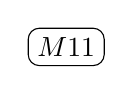
\begin{tikzpicture}\node[draw,rounded corners] {$M11$};\end{tikzpicture}}
a) $0$ et $1$ sont $\in R_0$ i.e. $\{0\},\{1\}\in\mathcal M_1$

b) $\forall A\in\mathcal M_2$, les fonctions
\[
 (x,y)\longmapsto x-y\qquad
 (x,y)\mathrel{\mapstochar\relbar}xy
\]
\deleted{c) $\forall A\subset R^*$, $A\in\mathcal M_1$, $\exists B\in\mathcal M_1$ tel que $A^{-1}\subset B$}
\margin{\deleted{(\unsure{car|OPS} OPS $B=A^{-1}$\,!)}}
sur $A$ sont modérées, \deleted{\unsure{car}} i.e. les deux parties de $R^3$
\[
 \{(x,y,x-y)\mid(x,y)\in A\},\qquad\text{et }\{(a,y,xy)\mid(x,y)\in A\}
\]
sont modérées.

c) $\forall A\subset R^*$, $A\in\mathcal M_1$, $\exists B\in\mathcal M_1$ avec $A^{-1}$ \deleted{modérée}\inserted{$\subset B$} (OPS $B=A^{-1}$\,!).

\deleted{Cet axiome} \deleted{\unsure{les parties a) b)}} \inserted{les parties a) b)} \unsure{équivalent|équivaut} à la validité de la

\margin{\uline{NB} Si $R\in\mathcal M_1$, il suffit de prendre $(M11)$ pour $A=R^2$}

\uline{Proposition} Pour un espace modéré $X$, les fonctions modérées $X\mathbin{-}R$ \deleted{\unsure{et|est} = une sous $R_0$} forment un \uline{sous-anneau} de l'anneau des fonctions scalaires sur $X$. En particulier, $R_0$ est un sous-anneau de $R$, et les anneaux
\margin{de fonctions mod. sont des $R_0$-algèbres}

\scanpage{22}
De $=$ pour $X$ un espace ind-modéré, p.ex. (si $R$ est réunion \deleted{des} de ses parties modérées $(M8)$ i.e. \inserted{les $R^I$} sont des espaces ind-modérés) pour les fonctions ind-modérées sur les $R^I$, qui contiennent en tous cas les \deleted{ensembles} anneaux de polynômes $R_0[(X_i)_{i\in I}]$ en les fonctions coordonnées.

\margin{Donc les applications $R_0$-polynomiales \deleted{entre} \deleted{transfont} $R^I$ sont modérées, et transfont des parties modérées en itou.}

\uline{Corollaire} Soit $f$ une fonction modérée sur l'espace modéré $X$. Alors $f$ est inv. dans l'anneau des fonctions modérées ssi $f$ ne s'annule pas dans $X$.

En considérant $f(X)\subset R^*$, cela revient au

\uline{Corollaire} Soit $A\subset R^*$, $A\in\mathcal M_1$, alors la restriction de $x\mathrel{\mapstochar\relbar}x^{-1}$ : $A$ est modérée, i.e. l'ens des $(x,x^{-1})\in R^2$, $x\in A$, est $\in\mathcal M_1$.
\mspage{21}

\scanpage{24}
\deleted{Si $x\in X\setminus Y$, $\exists\alpha$ tel que $f_\alpha(x)\ne0$, et}

définissent $Y$ comme l'ens des zéros communs. \deleted{de $X$} : ces fonctions, de plus elles séparent les pts de $X\setminus Y$, car si $x,y$ sont des pts distincts, \deleted{$\exists\beta$ tel que $f_\alpha(x)\ne0$ $g_\beta(x)\ne g_\beta(y)$ d'où}

Si les $f_\alpha$ \unsure{ne} suffisent pas à les séparer, montrons que les $f_\alpha g_\beta$ les séparent : en effet, $\exists\beta$ tel que $g_\beta(x)\ne g_\beta(y)$ \deleted{d'où} et $\alpha$ tel que $\lambda=f_\alpha(x)\ne0$, donc $f_\alpha(y)$ $(=f_\alpha(x)=\lambda\text{ par hyp.})\ne0$, d'où
\[
f_\alpha\underbrace{g_\beta(x)}_{\lambda}=\lambda g_\beta(x)\ne f_\alpha g_\beta(y)=\lambda g_\beta(y)
\]

Donc :

\uline{Proposition}. Si on a M1 : M\unsure{4|7} et M11, alors pour tt partie \deleted{\unsure{telle|fermée}} \inserted{modérée} $Y$ d'un esp. modéré $X$, qui est ens des zéros communs d'une famille finie de fonctions modérées sur $X$, on peut trouver une telle famille qui sépare les pts de $X$ (donc $X/Y$ est un espace modéré).

\mspage{23}

\scanpage{25}
À prouver

1) Si $X\to Y$ morphisme d'espaces modérés, $\exists$ partie modérée $Y'$ \uline{rare} dans $Y$ et
\[
(Z_i)_{i\in}\underbrace{\pi_0(Y\setminus Y')}_{I}=(U_i)_{i\in I},\quad Z_i\text{ modérés}
\]
\deleted{et des}
(de sorte que les $\overline U_i$ sont des parties modérées de $Y$) et enfin $\forall i\in I=\pi_0(Y\setminus Y')$, on ait une correspondance modérée
\[
R_i\subset(\overline U_i\times Z_i)\times X
\]
induisant une bijection entre $U_i\times Z_i$ et $X|U_i$ i.e. $X|\deleted{\unsure{(X\times_Y)}}U_i$ est fibré \deleted{loc.} trivial au sens modéré relatif ($U_i$ étant un espace modéré relatif \ldots)

Énoncé analogue pour un diagramme fini d'espaces modérés au dessus de $Y$ ??

Ce diagramme est ess.\textsuperscript{t} ``trivial par morceaux'' au dessus d'un $Y\setminus Y'$ convenable, avec $Y'$ modéré rare dans $Y$ ??? Ce serait déjà intéressant dans le cas particulier d'un diagramme de la forme $Z\subset X\subset Y\times\deleted{I}\inserted{[}0,1]$ \deleted{$\unsure{(I\subset[0,}$} au dessus de $Y$\ldots

\mspage{24}

\cotefile{136}
\scanpage{328}
4

\diagram{\begin{tikzcd}[column sep=large,row sep=small]
 & G_d \arrow[r,"\unsure{\sim}"] \arrow[d,dashed,no head] & G \arrow[d,dashed] \\
\mathbb Z \arrow[d] & \zeta_d \arrow[r] \arrow[d,no head] & \zeta \arrow[d] & \mathbb Z/2\mathbb Z \\
\zeta=\mathbb Z/2\mathbb Z & G_d \arrow[r,no head] \arrow[d,no head] & G=\mathrm{Sl}(2,\mathbb R) \arrow[d] \\
 & G'_d \arrow[r] \arrow[d,no head] & G'=\mathrm{GP}(2,\mathbb R) \arrow[d] \\
 & 1 & 1 \\
 & & H^2(X,\zeta)
\end{tikzcd}}

\figure{\begin{tikzpicture}[x=1cm,y=1cm]
\draw (0,0) .. controls (-.3,1.5) and (.4,3) .. (0,5);
\draw[->] (.45,1.7)--(-.3,1.1);
\draw[->] (.1,.4)--(-.65,-.25);
\draw (-3.4,-.1) .. controls (-3.2,-.65) and (-3,-.05) .. (-2.8,-.25)
 .. controls (-2.65,-.65) and (-2.7,-.55) .. (-2.2,-.45)
 .. controls (-1.9,-.4) and (-1.7,-.6) .. (-1.5,-.95);
\end{tikzpicture}}

\diagram{\begin{tikzcd}[column sep=small,row sep=large]
\zeta_u & H^2(B_G,\mathbb Z) \arrow[r,phantom,"\simeq"] \arrow[dl] & \mathbb Z\ni W \\
H^2(B_G,\unsure{\mathbb Z/2|\zeta}) & H^2(B_{G'},\mathbb Z) \arrow[u] \arrow[ddl] \arrow[ddddr,bend left=22] \arrow[r,phantom,"\simeq"] & \mathbb Z\ni\tfrac12 W \arrow[u,"2"] \\
\deleted{\unsure{\mathbb Z/2}}\cdot2=0 \arrow[u] & & \deleted{\unsure{\simeq}\,H^2(B_G,\pi)} \arrow[dll] \\
H^2(B_{G'},\zeta)\simeq\zeta\ni\xi \arrow[d] & & \\
H^2(B_{G'_d},\zeta) \arrow[d] & & H^2(B_{G'_d},\zeta_d) \arrow[ll,"\sim"'] \\
H^2(\pi,\zeta) & & H^2(X,\unsure{\mathbb Z|\zeta}
\end{tikzcd}}
\deleted{$\tfrac12 W\unsure{-|=}2g-2$.}

\diagram{\begin{tikzcd}[column sep=small,row sep=large]
\mathbb Z \arrow[d] \arrow[rrr,bend left=30] & H^2(X,\mathbb Z) \arrow[l,phantom,"\simeq"'] \arrow[d] \arrow[dr,phantom,"\text{Comm}" description] & H^2(B_{G'},\mathbb Z)\simeq\mathbb Z \arrow[l] \arrow[d] & W' \arrow[d] \\
\mathbb Z/2\mathbb Z & H^2(\unsure{X},\zeta) \arrow[d,leftrightarrow,"2"] & H^2(B_{G'},\zeta)\simeq\mathbb Z/2\mathbb Z \arrow[l] \arrow[d] & y \\
 & H^2(\pi,\zeta) & H^2(B_{G'_d},\zeta) \arrow[l] & \unsure{i}
\end{tikzcd}}

\diagram{\begin{tikzcd}
1\arrow[r] & \zeta\arrow[r,no head] & G\arrow[r,no head] & G'\arrow[r,no head] & 1
\end{tikzcd}}
\[H^2(B_{G'},\zeta)\]

\uline{\diagram{\begin{tikzcd}
X\arrow[r] & B_{G'_d}\arrow[r] & B_{G'}
\end{tikzcd}}}

\diagram{\begin{tikzcd}
H^2(B_{G'})\ni E'\arrow[r,"\sim"] & H^2(B_{T'})
\end{tikzcd}}

\diagram{\begin{tikzcd}[row sep=large]
X\arrow[r] & B_\pi\arrow[r] & B_{G'} & B_{\deleted{\unsure{T''}}\inserted{T'}}\arrow[l,no head] \\
 & \pi\arrow[r,hook] & \mathrm{GP}=G'\arrow[r,phantom,"\supset"] & S^1=T' \\
 & & \mathrm{Sl}=G\arrow[u]\arrow[r,phantom,"\supset"] & S^1=T\arrow[u,no head]
\end{tikzcd}}
\margin{$2g-2\ \text{ou}\ g-1$}
\margin{\diagram{\begin{tikzcd}
E''\arrow[r,mapsto] & 2g-2 \\
 & \sim\ g-1
\end{tikzcd}}}

\diagram{\begin{tikzcd}[column sep=small]
\mathbb Z\simeq\uline{H^2(X,\mathbb Z)} & H^2(\pi,\mathbb Z)\arrow[l,phantom,"\unsure{\simeq|\xleftarrow{\sim}}"'] & H^2(B_{G'},\mathbb Z)\ni E'\arrow[l,no head]
\end{tikzcd}}

\diagram{\begin{tikzcd}[column sep=small,row sep=large]
X\arrow[r] & B_\pi\arrow[r] & B_{G'} & B_{T'}\arrow[l,no head] & H^2(B_{T'},\mathbb Z)\simeq\mathbb Z\ni E'=\tfrac12 E\arrow[d] \\
 & & B_G\arrow[u] & B_T\arrow[l]\arrow[u] & H^2(B_T,\mathbb Z)\simeq\mathbb Z\ni E
\end{tikzcd}}

\mspage{329}

\scanpage{329}

\diagram{\begin{tikzcd}[row sep=large,column sep=large]
A\arrow[r,"u_{pq}"]\arrow[d,"u_p"'] & \Gamma^{pq}(\unsure{A|B})\arrow[d,"\gamma^B_{pq}"] \\
\Gamma^p(A)\arrow[r,"\Gamma^p(u_q)"'] & \Gamma^p(\Gamma^q(A))
\end{tikzcd}}

\diagram{\begin{tikzcd}
\Gamma^p\operatorname{Hom}(A,M)\arrow[d,no head] \\
\operatorname{Hom}(A,\Gamma^pM)
\end{tikzcd}}

\diagram{\begin{tikzcd}[column sep=large,row sep=large]
A\arrow[r,"f"]\arrow[d,"u_p"'] & \Gamma^{*}M \\
\Gamma^p A\arrow[r,"\Gamma^pf"] & \Gamma^p(\Gamma^e M)\arrow[r,no head] & \Gamma^e M
\end{tikzcd}}

\diagram{\begin{tikzcd}[column sep=large,row sep=large]
A\arrow[r,"f"]\arrow[d,"u_p"'] & J \\
\Gamma^p(A)\arrow[r,"\Gamma^p(f)"] & \Gamma^p(J)\arrow[r] & J
\end{tikzcd}}
\figure{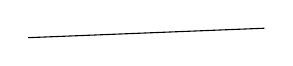
\begin{tikzpicture}\draw (0,0)--(3,.12);\end{tikzpicture}}

\unsure{Soit} $A$ une $k$-coalg co. unit. comm., de sorte que le foncteur $F_A(M)=\operatorname{Hom}_k(A,M)$
\diagram{\begin{tikzcd}
\mathrm{Ab}_k\arrow[r,"F",no head] & \mathrm{Ab}_k
\end{tikzcd}}
est muni d'une structure de quasi-commutation à $\unsure{\otimes}$ compatible avec \unsure{co. unit., comm.}).

\deleted{Conditions} \inserted{Données} équivalentes.

\textcircled{1} Donnée d'une quasi-commutation de $F$ aux foncteurs $\Gamma^p$, avec compatibilité aux $\beta_{pq}$ (structure multiplicative de $\Gamma$) et aux $\gamma_{pq}$ (structure \unsure{numér.|itérée}), enfin avec condition de comp. en degré $0,1$.

\textcircled{2} Donnée d'une famille d'élts
\[
u_p\in F_A(\Gamma^p(A)):\ A\mathrel{\relbar\joinrel\relbar}\Gamma^p(A)
\]
satisfaisant
\[
\begin{cases}
u_pu_q=C_{pq}\,u_{pq}\\
\Gamma^p(u_q)\circ u_p=\gamma^A_{pq}\circ u_{pq}
\end{cases}
\]
3 ie d'un hom \deleted{gradué} de $k$-alg. gr. divisées
\[
k\{T\}\xrightarrow{u}
\underbrace{\operatorname{Hom}(A,\Gamma^*(A))}_{\substack{\text{algèbre}\ \text{grâce à}\ \text{structure}\\
\text{de coalg. de }A\text{ et d'alg.}\\
\text{grde}\text{ de }\Gamma^*(A)}}
\]
satisfaisant
\[
\Gamma^p\bigl(u(T^{(q)})\bigr)\circ u(T^{(p)})
=\gamma^A_{pq}\,u(T^{(pq)})
\]

\mspage{330}
